% NEWSECTION ===================================================================
\section{Introduction} % status: need Lidar comparison, etc
This thesis was performed alongside work and research done for the SMART3D project. The SMART3D project originally started in 2016 as an investigation into the feasibility of using a Photonic Mixing Device (PMD) sensor as an alternative to lidar in detecting 3D objects in short-range outdoor applications. Over the course of the project, a shift was made from PMD sensors to stereo cameras, and thus began the topic of this thesis. This work seeks to address and answer the how well a stereo-based 3D object detector performs, especially in comparison to lidar, the natural and primary choice for estimating an object's location in an outdoor environment (such as detecting other cars on the highway). Stereo vision, specifically on vehicles, typically consists of a 2-camera setup using passive color light detection to generate an estimated stereo disparity map. This may then be transformed into a point cloud and subsequently analyzed with a Pointnet object detector. In this thesis, the performance of such a system, or network as they are known, is evaluated as well as compared with that of similar detection networks.

% so, need to figure out what the general order of this paper will be. let's try the following: \\
% stat | descrip
% done | 1.0 introduction \\
% inpr | 1.1 problem / motivation
%      | 1.2 requirements
% inpr | 2.0 related work \\
%      | 3.0 Short overview of components in stereo network \\
%      |   3.1 psmnet and stereo estimation networks \\
%      |   3.2 mathematics of stereo 3D reconstruction \\
%      |   3.2 pointnet and pointnetworks \\
%      | 4.0 general steps of spnet (stereo point net) \\
%      |   4.1 stereo estimation (performance, results) \\
%      |   4.2 stereo 3d reconstruction (performance, results) \\
%      |   4.3 stereo point net (procedure, modifications, performance) \\
%      | 5.0 results of stereo point net \\
%      | R. references \\
% done | A. PerformanceMetrics \\
% done | B. About the KITTI Dataset \\
% done | C. Lidar vs Other Sensors \\


\subsection{Motivation}
The field of artificial intelligence has exploded in recent years, in part due to the usage of convolutional neural networks (CNN's) and the usage of graphics processing units, GPU's. This has enabled further research into systems that can quickly understand their surroundings, having applications in other fields, one of which is autonomous driving. The subfield of autonomous driving has seen great success in the application of camera data for 2D localization. However, driving is a process that requires some 3D knowledge, which means the usage of lidar has followed the growth of this sub-field. To its credit, lidar is a technology with multiple benefits: a lidar scan is precise, works outside, works in darkness, and provides immediate metric information about the world. Unfortunately, lidar sensors also have the disadvantage of being rather expensive when compared to passive sensors such as cameras. In this context, expensive means the relative amount of usable information that is output at a standardized rate per amount of money spent. There are a few factors to normalize, and a more in-depth analysis of this is conducted below. In addition to the high cost, there may be other hidden disadvantages of using lidar, such as a weaker or missing return signal on reflective surfaces, potential interference of multiple lidar sensors if they're all in the same area (e.g. multiple autonomous vehicles at an intersection), and the relatively slow refresh rate lidar sensors can achieve when compared to passive sensing cameras. Therefore, despite lidar being a worthy technology of use, this paper seeks to explore an alternative technology, stereo vision, to estimate the 3D positions of objects.

There are some interesting benefits that may be gained with stereo vision, because stereo cameras: are relatively cheap for the amount of information they provide, intuitively mimic the way that humans already perceive and navigate their world, are passive sensors that do not interfere with other sensors, and have a high refresh rate (dependent on the camera system, but 10 FPS, ``frames per second", is around the lowest value for any camera). Of course, using a stereo vision system is not without downsides, including: inability to function at night without adequate lighting, difficulty understanding large texture-less surfaces, and an error that increases quadratically with distance. This last points simply means that as the distance of an estimated point increases, the error of that value increases quadratically, as mentioned by \cite{wang_pseudo-lidar_2019} and visualized below in Figure xx (need correlation beteween lidar distance and stereo disparity).

% lidar economics part here
\def \deg {$ ^{\circ}$\ } % need extra backslash for space

Lidar dominates the environmental sensing space for some very good reasons. It is primarily used for its accuracy at intermediate distances, in the 5-100 meter range. It also is capable of sensing in a 360\deg field of view, and can continue detection during low-light conditions. However, as described by \cite{broggi_sensors_2013}, most modern lidar sensors have a rolling shutter, which causes deformation in the data to correct. They also typically cost much more than a stereo camera system, require moving parts (thus becoming sensitive to vibration), and the other reasons mentioned previously.
% In terms of low visibility conditions, such as rain or fog, both cameras and lidar sensors suffer a performance decrease, but stereo cameras are more robust as there must be significant weather conditions to deteriorate their vision, similar to how humans may navigate through poor weather.

In order to make a more quantitative comparison between these two ranged sensing methods, the hardware setup used in the KITTI dataset will be analyzed. In collecting the necessary information to create the various datasets, \cite{geiger_are_2012} used a Velodyne HDL-64E lidar and two PointGrey Flea 2 color cameras. In 2012, when the paper was first published, an HDL-64E cost in the range of 75.000 USD (US dollars) xx. Although exact price information for the cameras, which have been discontinued, is difficult to find, a similar model (FL2-03S2C-C) seems to have been priced around 700 USD for a single camera; the two-camera system will therefore be assumed to have cost 1,400 USD xx. Although this clearly demonstrates that the cameras are cheaper, an attempt to normalize for point cloud density / quality will be made next. See Table \ref{economics_table} below for more information on both sensor setups.

A numeric comparison may be made between sensors, in an attempt to correctly account for several features that one may have while the other may not. Ideally, one would want to have both a high quantity of information as well as a high quality of information. To start, the ``quantity" argument will be examined. Because lidar has 360\deg vision and cameras do not, the camera price and points per scan will be multiplied by four to simulate having cameras on each side of the car, thus simulating near-360\deg vision of the environment (although in the end this does not affect any ratios). Additionally, from scan to scan in the KITTI dataset, there is a varying number of points in the lidar point cloud. Thus, an average of the number of points in each lidar scan was obtained.

A quick note about the camera FOV (field of view): although the stated raw FOV is 90\deg by 35\deg, there is some angular reduction due to both rectification and cropping necessary to standardize image sizes for disparity calculation. Thus, it will be assumed that although a single stereo camera system does not have it's original FOV dimensions, it may have at least 90\% of the original values.

\def \b #1{\textbf{#1}}
\begin{table}[ht]
	\centering
	\caption{Economic comparison of KITTI dataset sensors, including a theoretical four-system stereo setup. hFOV refers to ``horizontal field of view", vFOV for vertical, cost is in estimated US dollar price in 2012, points/scan refers to how many points a sensor provides for each scan, and angular area is in ``square radians" (elaborated below), describing the visible area based on a sensor's vertical and horizontal FOV's. The ``Stereo (x4)" column simulates as-if a single stereo setup were to be used to obtain near-360\deg vision of the environment, imitating lidar.}
	\begin{tabular}{|c|c|c|c|}
	\hline
	\b{Property}              & \b{Lidar} & \b{Stereo (x1)} & \b{Stereo (x4)} \\ \hline
	hFOV (deg)                & 360       & 81              & 324       \\\hline
	vFOV (deg)                & 20,0      & 31,5            & 31,5      \\\hline
	Cost (USD)                & 75.000    & 1.400           & 5.600     \\\hline
	Points/Scan               & 476.898   & 453.376         & 1.813.504 \\\hline
	Angular Area ($rad^2$)    & 2,18      & 0,77            & 3,07      \\\hline
	Points/Price (pts/USD)    & 6,36      & 323,84          & 323,84    \\\hline
	Points/Area (pts/$rad^2$) & 218.761   & 588.800         & 588.800   \\\hline
	\end{tabular}
	\label{economics_table}
\end{table}



To properly clarify the table, ``angular area" will be explained. Angular area, solid angle, square degrees, etc, is a value in ``square radians" ($rad^2$) describing the visible region from a given viewpoint. Solid angle may be defined as given in Figure \ref{eq_solidangle1}.In this equation, $A$ is the spherical surface area, and $r$ represents the sphere's radius. Given that a sphere's surface area is $4\pi \ rad^2$, the maximum theoretical solid angle any sensor may have is $4\pi$, or about 12.57 square radians. However, since only vertical and horizontal field of view are given, the formula to calculate solid angle is then modified to Equation \ref{eq_solidangle2}. Here, $\theta$ and $\phi$ represent the horizontal and vertical field of view (FOV), respectively. The spherical coordinate system used along with an example graphic is shown in Figure \ref{solidangle}. As an example, the lidar system, with hFOV of $[0,360]$ degrees and vFOV of $[-10,10]$ degrees, may thus be calculated to have an solid area of about 2.18 ${rad}^2$ (previous values automatically converted).

\begin{equation}
\Omega = \frac{A}{r^2}
\label{eq_solidangle1}
\end{equation}

\begin{equation}
\Omega =
\frac{1}{R^2} \int_{\theta} \int_{\phi} R^2\cos(\phi) d\theta \phi =
(\theta_{b1} - \theta_{a1})[\sin(\phi_{b2}) - \sin(\phi_{a2})]
\label{eq_solidangle2}
\end{equation}

\begin{figure}[ht]
    \centering
    \subfigure[Solid angle coordinate system]{
        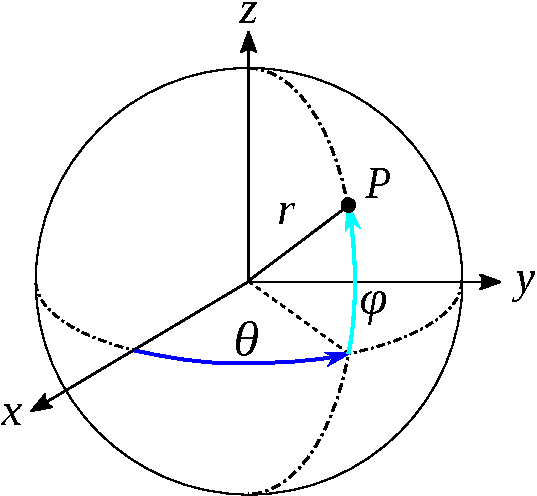
\includegraphics[width=0.35\linewidth]{../media/solidangle_cs.pdf}}
    \subfigure[Solid angle example graphic]{
        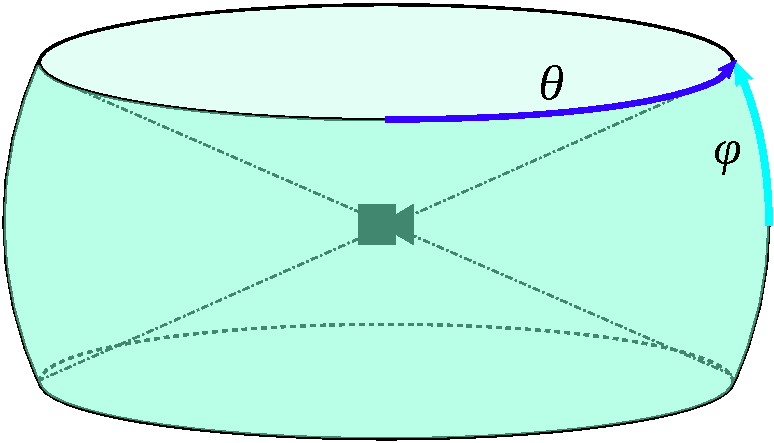
\includegraphics[width=0.5\linewidth]{../media/solidangle_ex.pdf}}
    \caption{(a) Spherical coordinate system for Equation \ref{eq_solidangle2}. (b) Example graphic demonstrating where angle values correspond to sensor. The transparent green region represents the sensor's visible field.}
    \label{solidangle}
\end{figure}

Given the information above, stereo sensors are the clear winner in terms of points per dollar (points/price) as well as point density (points/area).

On the question of quality, lidar becomes the de facto standard of measure due to its high accuracy.
This means that stereo vision quality is derived from how closely it matches a lidar scan. This also means that stereo vision quality is highly dependent on the system used, and can vary with both hardware and software implementation. A typical engineering threshold of 10\% is used for comparison, meaning that a single stereo-generated point is considered ``good" if its depth estimate is within $\pm$10\% of the absolute value of the corresponding lidar depth estimate. The horizontal and vertical distances, $x$ and $y$, are ignored due to the assumed 1:1 correspondence when projecting a point cloud onto the image plane. The steps to determine this quality are:

\begin{itemize} \itemsep=-0.5em
    \item Project lidar points to image space, named $L$
    \item Convert disparity values of stereo map to depth values, named $S$
    \item Keep only points from stereo map that also exist in $L$
    \item For each $(i=row,j=column)$ index, obtain the lidar distance, stereo distance, and the absolute error between them as:
\begin{equation}
    e = \left | \frac{S_{i,j} - L_{i,j}}{L_{i,j}} \right |
    \label{eq_errCalc}
\end{equation}
    \item Tally how many points fall within the $\pm$ 10\% threshold as a percentage of the total points.
\end{itemize}

After performing the following steps, Figure \ref{corr_disp_lidar} was generated: A lidar-stereo graph that merely indicates at what distance value a given stereo point has, and what value its corresponding lidar point also has.

\begin{figure}[ht]
	\centering
	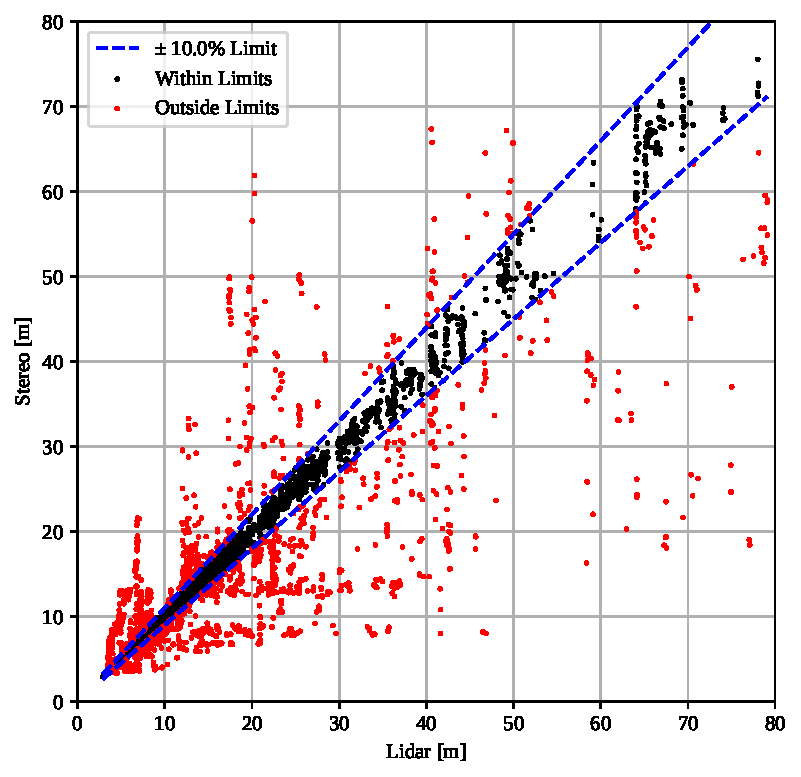
\includegraphics[width=0.6\linewidth]{../media/corr_stereo_lidar.pdf}
	\caption{A visual correlation between lidar and stereo depth values that have been projected onto the image plane, removing the need to correlate horizontal or vertical distances. The more points that lie within the $\pm$10\% limit, the better that stereo depth maps approximate lidar point clouds. Pearson correlation coefficient between Lidar and Stereo data is 0.927. Stereo data was generated using a modified Pyramid Stereo Matching network, described in Section xx. Lidar data was taken from the KITTI Object Detection dataset.}
	\label{corr_disp_lidar}
\end{figure}

In summary, stereo vision is an attractive alternative to lidar vision because of its much higher point density, lower price, reasonable quality approximation of lidar, and the potential to improve through further research. Under the correct conditions, stereo vision sensors have the potential to compete with lidar sensors in terms of both quantity and quality.

HDL-64E:
range: 120 m
pts/s: 1,000,000/s (10Hz)
cost: \$85,000 (2017)

%https://www.velodynelidar.com/lidar/products/manual/HDL-64E%20Manual.pdf
%https://medium.com/self-driving-cars/velodyne-lidar-price-reduction-d358f245f086
%https://driverless.wonderhowto.com/news/quanergys-new-250-solid-state-lidar-could-bring-self-driving-masses-0175790/




\subsection{Requirements}
In order to develop a stereo-based 3D estimation algorithm and conduct a performance comparison, there are multiple needs that must be met. The very first need that must be met is a dataset that contains all the necessary information for a lidar-based network to detect objects, as well as a stereo-based network. For this reason the KITTI dataset, a well-known and actively used benchmark, was selected as the source of data to compare the two technologies.


\subsection{Project Background}
This thesis and project was born out of the SMART3D project, and thus the two have similar but slightly different goals. It must also be noted that an important and relevant paper was published by \cite{wang_pseudo-lidar_2019} during the time the SMART3D project had already begun and before the completion of this thesis. This means that although the inspiration for stereo-based 3D object estimation came from two separate sources, this paper is technically following in similar footsteps, and indeed draws some ideas from the ``Pseudo-LiDAR from Visual Depth Estimation" paper. The overlap and inspiration from the two will be acknowledged when appropriate throughout this paper.

The SMART3D project itself is an investigation into short-range, outdoor sensor alternatives to lidar, originally based around PMD sensors. However, there was eventually a switch to passive stereo vision because of the missing available dataset at the time. Thus, the desire to use stereo vision came from an initial goal of finding a reasonable alternative to lidar for short-range outdoor sensing applications.

% NEWSECTION ===================================================================
\newpage
\section{Related Work} % status: stereo vision, 3D, etc

\subsection{Stereo Vision}
Stereo disparity maps, which are built by the comparing the pixel distance between two similar regions of two images, have existed before the implementation of artificial intelligence to create them. Famously, \cite{scharstein_taxonomy_2002} gave a taxonomy and categorization of the various aspects of stereo vision. Out of this paper, the four main parts of conducting stereo vision have been classically defined as follows: matching cost computation, cost (support) aggregation, disparity computation and optimization, and disparity refinement.

Initially, built-in and readily available stereo disparity map computation techniques were used. In the Python OpenCV library, there is a ``Semi-global Block Matching" (SGBM) algorithm, implemented based on the paper by \cite{hirschmuller_stereo_2007}. For an initial ``rough" pass, this algorithm was cheap and fairly effective. Additionally, this algorithm is useful for fast, fairly-stable calculations and does not need a GPU to run. However, it suffers from a few key shortcomings. For one, there is a large portion of the disparity map that contains no values, as can be seen below in Figure \ref{ind15_SGBM_comparison}. Next, when a set of pixels cannot be matched between images, the result is simply a NaN result, giving no information in that region. Finally, SGBM suffers from some significant lack of resolution, meaning that some objects of interest, such as the three pedestrians image, will not be seen well, or at all. For comparison, stereo images created with a neural network (NN) such as those in Figure \ref{new_psmnet} have a richer amount of information and have no missing pixels (i.e. a prediction is made at every pixel).

xx NEED TO TALK ABOUT WHY STEREO RCNN ISN'T THE BEST WAY TO GO


\begin{figure}[ht]
    \centering
    \subfigure[SGBM disparity map]{
        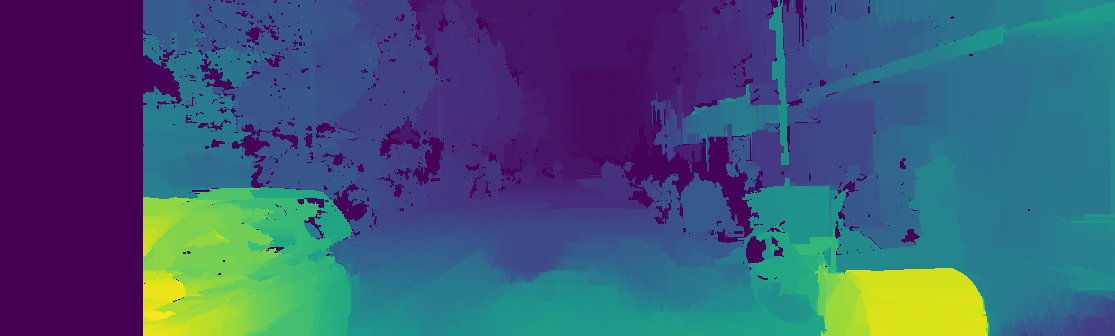
\includegraphics[width=1\linewidth]{../media/ind15_SGBM_comparison.png}}
    \subfigure[LHS image]{
        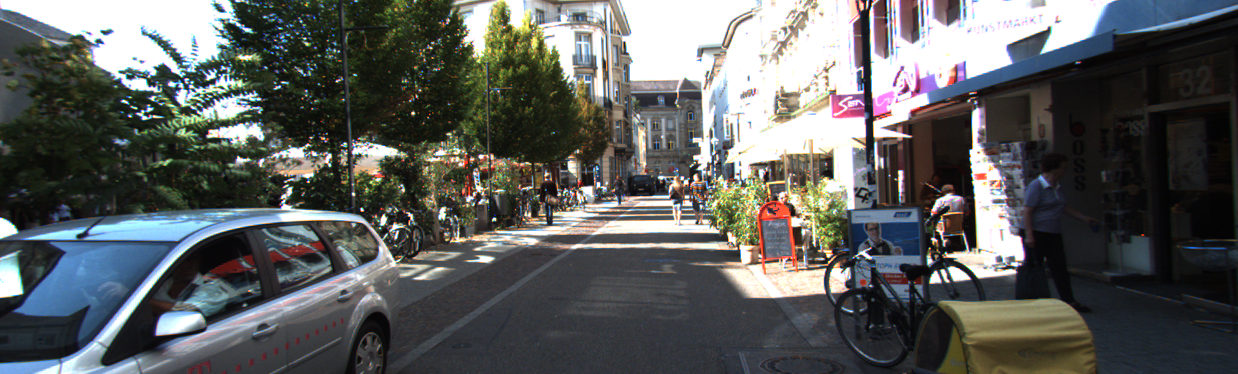
\includegraphics[width=0.487\linewidth]{../media/objdet_LHS_000015.png}}
    \subfigure[RHS image]{
        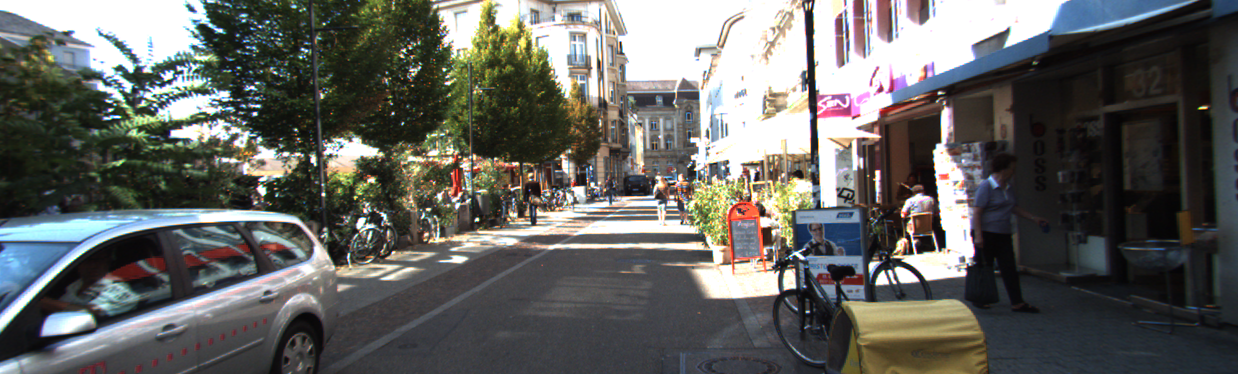
\includegraphics[width=0.487\linewidth]{../media/objdet_RHS_000015.png}}
    \caption{An example of a disparity map generated without a neural network approach. Though It has good merit, there are some noticable shortcomings. Disparity map generated by image pair shown below. Index 15.}
    \label{ind15_SGBM_comparison}
\end{figure}


With this knowledge, the next step was to find an ideal NN-based stereo disparity estimation method. Notable neural network approaches to disparity estimation include Pyramid Stereo Matching network (PSMnet),  iResNet, and even some monocular-based approaches including one used by Wang et al. named DORN, by  \cite{fu_deep_2018}. In order to select the best candidate, multiple benchmarks were considered. The first benchmark was naturally the KITTI Stereo challenge, which contains a list of the top performing networks. At the start of this thesis writing, PSMnet stood in the top 10 of stereo networks in this list \cite{menze_kitti_2019}.

Pyramid Stereo Matching Network, or PSMnet, is a network that takes advantage of an hourglass-shaped network. It is super cool because it produces these very high quality, high resolution disparity maps. The network takes advantage of GPU processing power, depending on nVidia's GPU acceleration, similar to other networks. The network itself is written in PyTorch, a flexible and python-based network module. The use of PyTorch enabled fast, simplified debugging. PSMnet's architecture is shown below in Figure \ref{psmnet_arch}.


\begin{figure}[ht]
    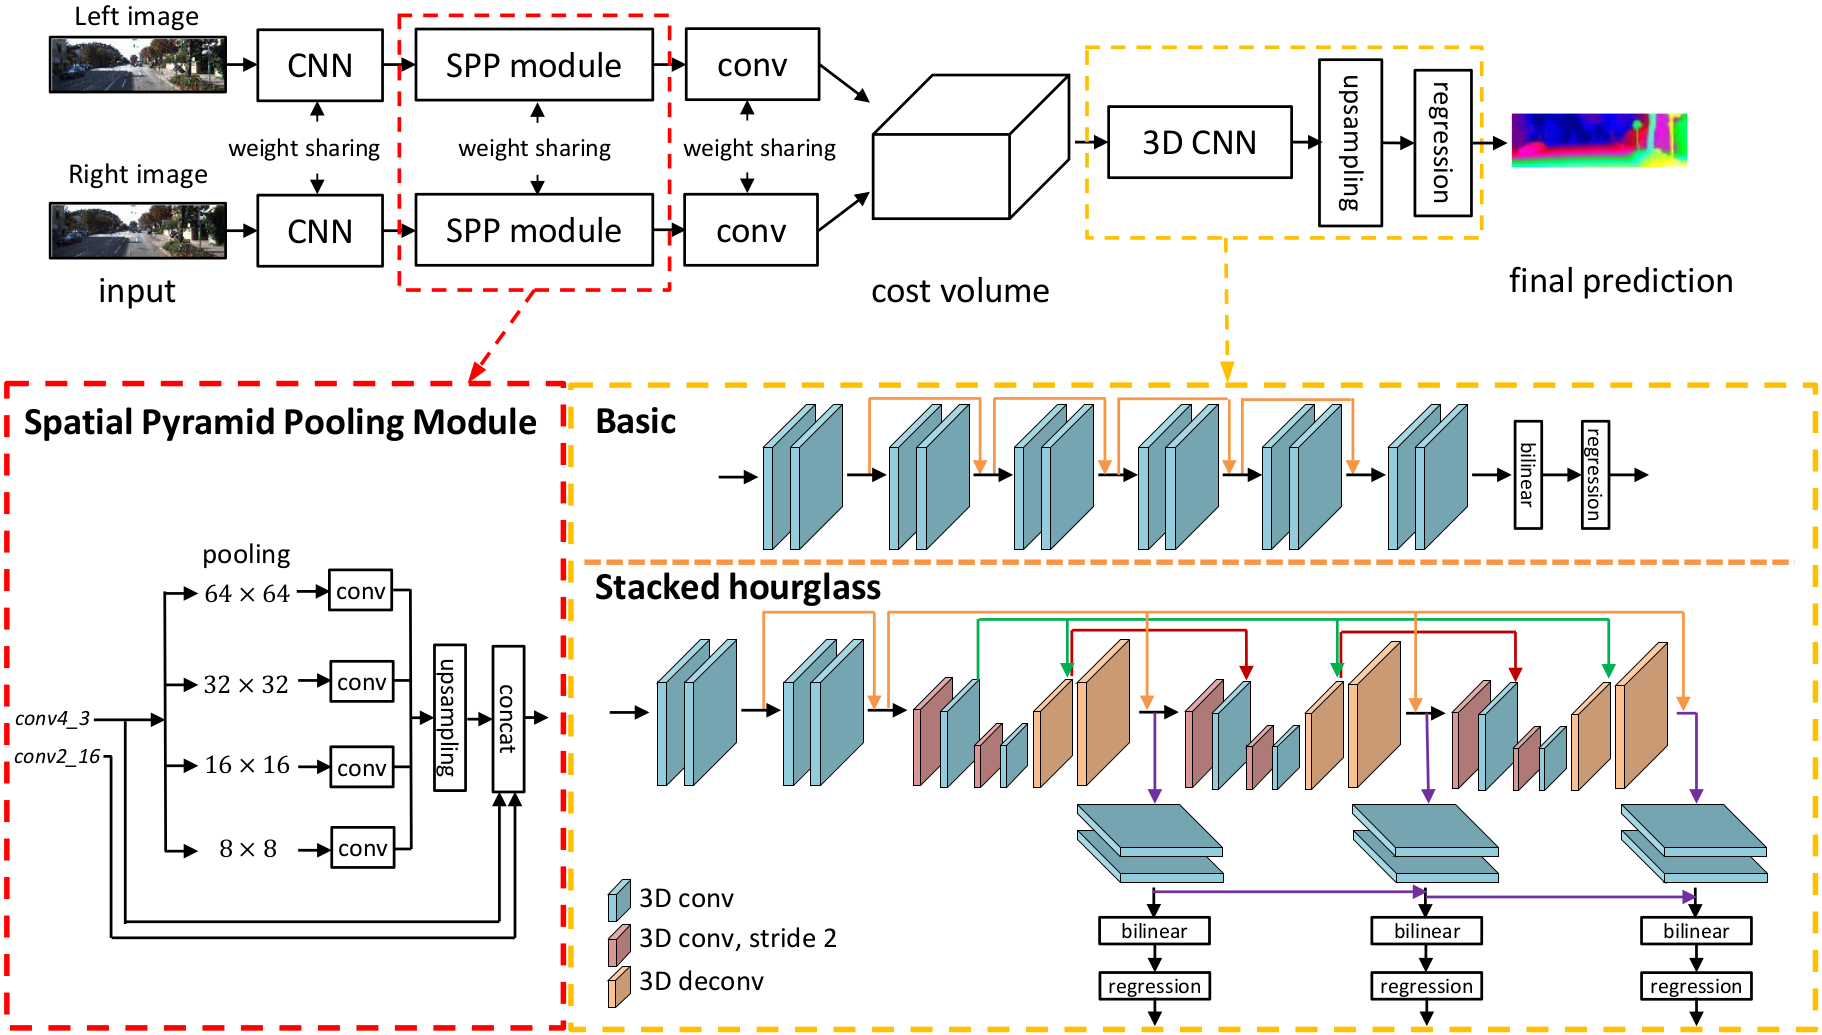
\includegraphics[width=1\textwidth]{../media/psmnet_arch.png}
    \caption{Generalized network architecture for Pyramid Stereo Matching network. The 3D CNN has two available configurations, Basic and Stacked hourglass. Stacked hourglass was used here. The Spatial Pyramid Pooling Module helps describe how features at varying ``zoom" levels were concatenated together. Image reproduced from \cite{chang_pyramid_2018}.}
    \label{psmnet_arch}
\end{figure}

\subsection{3D estimation with Stereo Disparity Maps}
There is a surprisingly low amount of public research on stereo vision for use with 3D localization. \cite{li_stereo_2019} created an RCNN-based approach that currently performs best in class on the KITTI dataset, although achieving 59'th place when also compared against networks that use lidar. This paper also cites other works, such as ``3DOP" by \cite{chen_3d_2016}. However, some prior information is encoded into the calculation before using regression to estimate object pose, including height above ground, object size priors, and ``depth informed features", while our paper does not provide this information to the network beforehand.

A recent development has been published since the start of this paper, by Wang et. al. In their paper, ``Pseudo-LiDAR from Visual Depth Estimation" \cite{wang_pseudo-lidar_2019}, the authors took an extremely similar approach to this paper. Their pipeline / steps, outlined below in Figure \ref{pseudonet_arch}, was to take a stereo image pair, generate a disparity map via Pyramid Stereo Matching network, convert it to a ``pseudo-lidar" scan, and extract 3D bounding box estimations via Frustum Pointnet. \\

\begin{figure}[ht]
    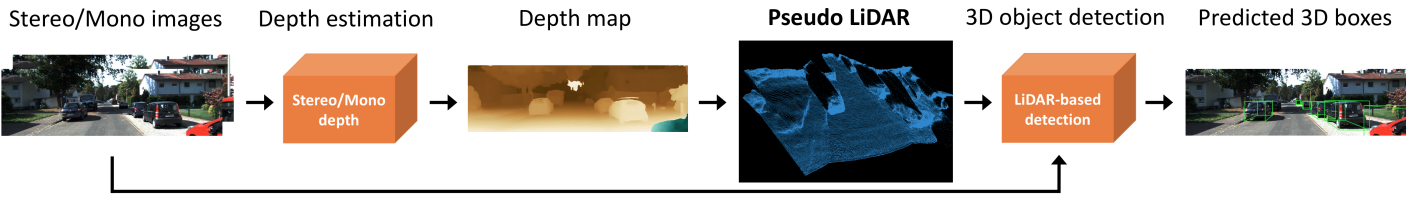
\includegraphics[width=1\textwidth]{../media/pseudonet_arch.png}
    \caption{Architecture of the Pseudo-LiDAR network. Stereo (or mono) image data is used to create a disparity map, which is converted to lidar, and is then used by a 3D detector to estimate 3D bounding boxes.}
    \label{pseudonet_arch}
\end{figure}

In their paper, the authors argue that within a short distance, up to 30 meters away, stereo vision performs competitively with lidar.

XX NEED TO MENTION AVOD A LITTLE BIT AND EXPLAIN WHAT IT IS

\subsection{3D Estimation with Lidar}
Performing 3D estimation and localization with lidar has been a focus for a large portion of the field, and with good reason. Thus, there are many papers which focus on using lidar sensor capabilities to estimate 3D bounding boxes, to varying degrees of success. \cite{qi_frustum_2017} paper, currently one of the best performing networks, forms a part of the work of this research paper as well.

\subsection{3D Reconstruction with Stereo Data}
\label{sect_reconstruct}
3D reconstruction from a disparity map can be performed multiple similar but slightly different approaches. Regardless of the approach, the goal is to end up with a pointcloud, an unordered set of metric coordinates. The first approach, working with epipolar equations, is the most intuitive. The second, remapping the projected 2D points back into 3D space, is equally effective, but only used to map lidar points onto the image plane (the reverse of reconstruction). \cite{szeliski_computer_2010} goes into some detail over the first method, which principally deals with the high level equations necessary to generate each (x,y,z) coordinate.

The first approach, using epipolar equations, can be described in general as follows. First, some necessary assumptions:
\begin{itemize} \itemsep=-0.5em
    \item The camera centers are aligned (for simplified rectification).
    \item Images are already rectified (to remove all distortion).
\end{itemize}

Given the above, there must first be a given disparity map image, $D$, with indices ($u$,$v$) corresponding to the image's x-axis and y-axis (origin located at the top-left of the image). The cameras' intrinsic properties must also be known (P2 for the KITTI dataset), as well as the baseline, $b$, distance (also known as the distance between camera centers). In the KITTI dataset, Camera 2 is the LHS color camera, and thus each record's corresponding P2 matrix is used. The matrix contains the horizontal focal length $f_U$ as well as the vertical focal length $f_V$. \cite{szeliski_computer_2010} describes this in Equation 2.57 of Chapter 2: Image Formation. The camera baseline is given in multiple locations, namely \cite{geiger_are_2012}, although the value is given as ``roughly 54 cm", which may reduce the overall accuracy somewhat.

Given this data, the depth value at each pixel location may be calculated via Equation \ref{eq_epi_z}, ignoring locations where the disparity value is 0 or Not-A-Number (NaN).

\begin{equation}
z = \frac{f_U * b}{D}
\label{eq_epi_z}
\end{equation}

Next, the real-world $x$ and $y$ locations may be calculated by taking the relative coordinate location from camera center $(c_U,c_V)$, multiplying by the depth values at each pixel location. Successfully calculating this leads to an estimated metric coordinate value for every valid pixel disparity value in the image.

\begin{equation}
x = \frac{(u - c_U) * z}{f_U}
\end{equation}

\begin{equation}
y = \frac{(v - c_V) * z}{f_V}
\end{equation}

In reality, the calculation is performed in a series of matrix calculations rather than as an element-by-element operation. The ``real" steps taken to convert a disparity map into a pointcloud are described in Appendix \ref{appendix_reconstruct}.


% NEWSECTION ===================================================================
\newpage
\section{Development of 3D Estimation Network}
The 3D object detection network can be broken up into three main sections, as shown below in Figure xx.



\subsection{Modification of Pyramid Stereo Matching Network}
The first task in creating a network that can take a stereo image pair and generate 3D bounding boxes, as described in figure xx above, is to have the capability of taking a stereo image pair and creating a 2.5D disparity map. To that end, a best-in-class disparity generation algorithm was searched and was selected to be the Pyramid Stereo Matching Network. Pyramid Stereo Matching Network was published by Jia-Ren Chang and Yong-Sheng Chen in March 2018. This network takes a deep learning approach to generating disparity maps from a pair of images. The network itself is near the top of the state of the art, and achieves this by the architecture of its network. (xx architecture and style need to be elaborated upon in the ``related work" section). The openly-available repository provided a foundation to start on towards making a compact, easy-to-use function.

First, the original evaluation code was tested out. Some modification and housekeeping had to be done to ensure that it was compatible with the local installation, as well as being adapted for use with Python 3. All deprecated functionality was manually removed.

\subsubsection{Similarity of Ground Truths Across Datasets}
After the initial evaluation, the network was prepared for and trained on KITTI data. I first downloaded the network that was pre-trained on the Freiburg SceneFlow dataset, available from the PSMnet authors. Next, I finetuned the network by training it on KITTI data. Here, it must be clarified that there are images in the KITTI stereo dataset that overlap greatly in similarity to those in the KITTI object detection dataset. The difference between the two datasets are essentially that one has been optimized for object detection, and the other for stereo disparity map estimation. This similarity was also noted in \cite{wang_pseudo-lidar_2019}, and I took the same approach to correct it, as described below.Figure \ref{similarity_stereo_objdet} below also demonstrates the similarity between two sample images, which leads to the problem of having a part of the network trained on what may be validation or even evaluation data.

\begin{figure}[ht]
    \centering
    \subfigure[000132\_10 from Stereo]{
        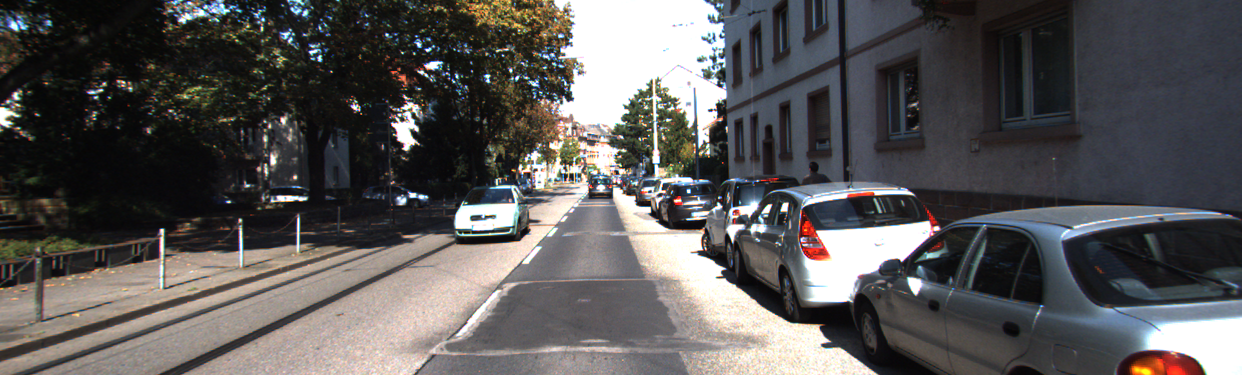
\includegraphics[width=1\linewidth]{../media/similar_000132_10_stereo.png}}
    \subfigure[000286 from ObjDet]{
        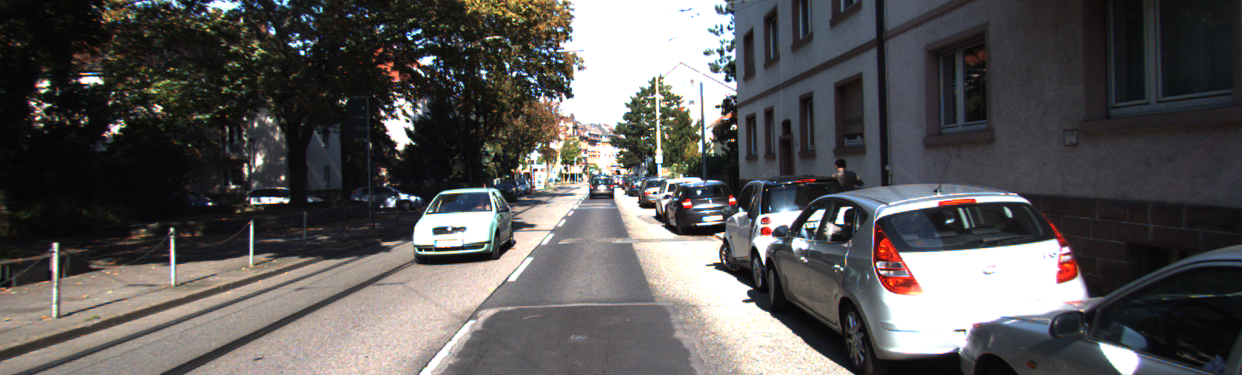
\includegraphics[width=1\linewidth]{../media/similar_000286_objdet.png}}
    \caption{Example of how two unique records from the separate datasets have overly-similar scenes. There are multiple examples of this, which creates the motivation to generate a secondary set of disparity ground truths for the object detection dataset}
    \label{similarity_stereo_objdet}
\end{figure}

In order to deal with the dataset overlap, the KITTI object detection dataset was adapted to be used for training stereo data. Lidar data was projected onto the LHS image plane, converted to integer values, then multiplied by a constant. These steps are in line with both the way that [xx] were able to generate their self-made stereo ground truths as well as how the KITTI dataset authors generated their ground truth [xx reference to devkit]. Locations in the image that have no lidar data are left alone at a value of 0.0, and finally the resulting array is saved to a PNG image file format containing integer values. Please refer to the generation script in the repository for the exact steps used to generate the pseudo ground truth stereo images.

\subsection{Retraining PSMnet with Object Detection Data}
It was discovered at some point that the training / validation data used in the KITTI stereo image set was overlapping too much with images used in the KITTI object detection task. Thus, \cite{wang_pseudo-lidar_2019} was referred to and guided the change in retraining PSMnet. The difference in training is shown below.

Figure \ref{psmnet_star_train_info} below shows the loss throughout the training of PSMnet on the object detection dataset, also known as PSMstar (based on the similar name given in Wang et al's paper), as well as the original stereo dataset model for reference. It should be noted that validation error



\begin{figure}[ht]
    \centering
        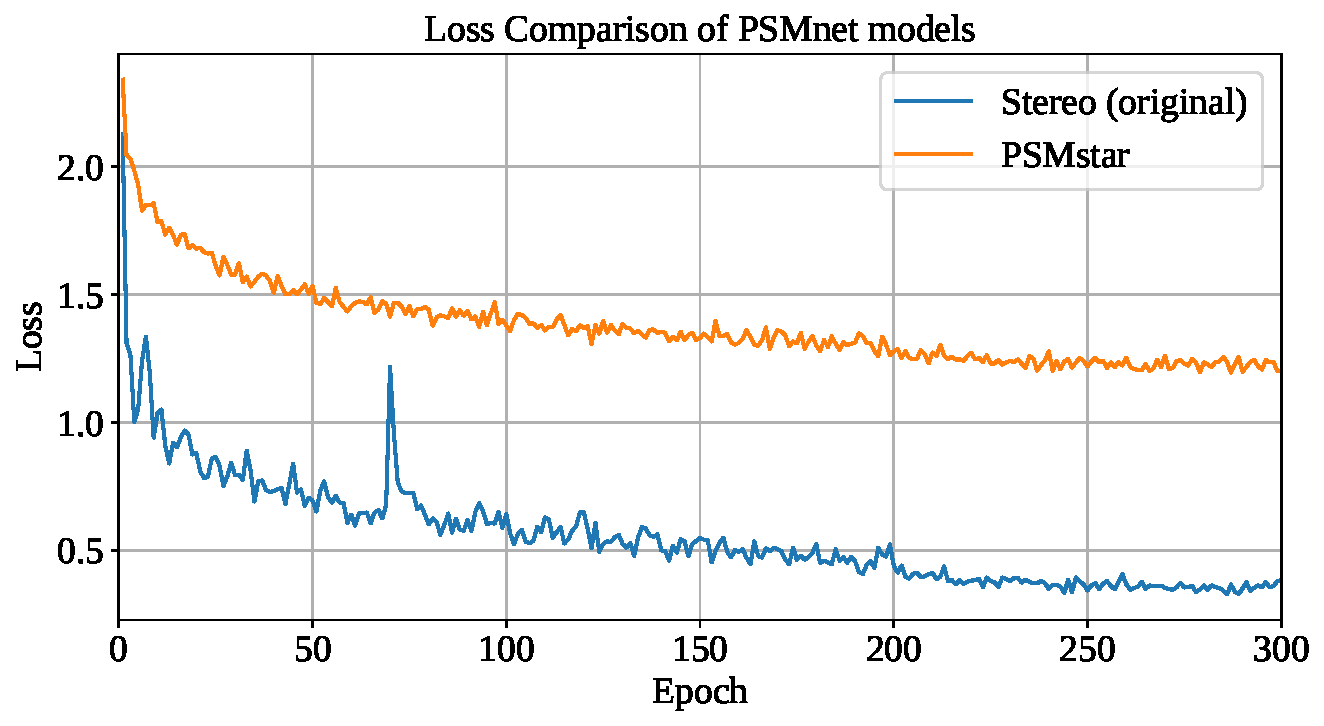
\includegraphics[width=0.9\linewidth]{../media/info_psmnet_comparison_Loss.pdf}
    \caption{Loss graphs for both the original stereo-dataset PSMnet model and the retrained, object-detection-based ``PSMstar" model. The average difference between the two curves is a loss of about 0.82. The higher loss for PSMstar may result from using self-made ground truth labels rather than using the more detailed stereo dataset versions.}
    \label{psmnet_star_train_info}
\end{figure}

In addition to the quantitative difference in training, a qualitative difference in the estimation pattern may be seen below, in Figure \ref{new_psmnet}. Overall, the change in quality may be seen as a more detailed but less contrasting depth map.

\begin{figure}[ht]
    \centering
    \subfigure[Stereo estimation with original PSMnet model]{
        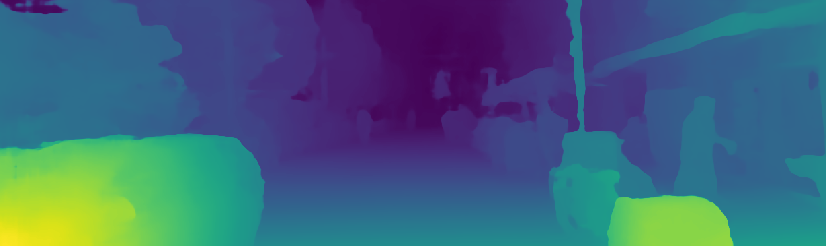
\includegraphics[width=1\linewidth]{../media/ind15_psmnet_v190308_AsOf190626.png}}
    \subfigure[Stereo estimation with new PSMnet* model]{
        
\includegraphics[width=1\linewidth]{../media/ind15_psmstar_v190613_AsOf190626.png}}
    \caption{Comparison of old and new model for PSMnet. Index 000015. [xx add more detail]}
    \label{new_psmnet}
\end{figure}



\subsection{Development of Stereo 3D Reconstruction Function}
As described in Section \ref{sect_reconstruct}, the overall steps of reconstructing the resulting stereo image consisted of three general equations adapted for use with matrix operations. This also included selecting the proper constants for each calculation. To achieve all this, a specific class was created that would initialize by loading the fully trained model and use it in a non-learning ``testing" mode, whereby it would take in either an image path pair or a loaded pair of image arrays. The pair would then be evaluated in PSMnet, which returns a stereo map, and finally be converted to a pointcloud using the epipolar equations in matrix form. Each record of the KITTI dataset has its own calibration file, but the baseline value remained the same. During the overall Frustum Pointnet training and evaluation, a new pointcloud would be generated in real-time.

\subsection{Modification of Frustum Point Net}
Frustum Pointnet, being originally written for Python 2, needed to undergo some minor adaptations while being modified for usage with Python 3. For example, several modules and functions were deprecated or needed modification, and so had to be properly adapted. There are also two actively maintained versions of the frustum Pointnet code. as explained in the original paper [xx], there are two versions of the FPNet model: the first which uses standard Tensorflow libraries, and the second which uses custom Tensorflow operators that must be compiled. For the purposes of this paper, version 1 was used and will be the default version unless otherwise noted.

In order to transition from using the provided pre-trained model and preprocessed data to self-made preprocessed and trained data, a set of steps and ``paths" were created to guide what was happening in each step and set of ``runs". As shown below in Figure \ref{fp_paths}, there are various steps with gradually increasing dependence on stereo-based pointcloud data.

\begin{figure}[ht]
    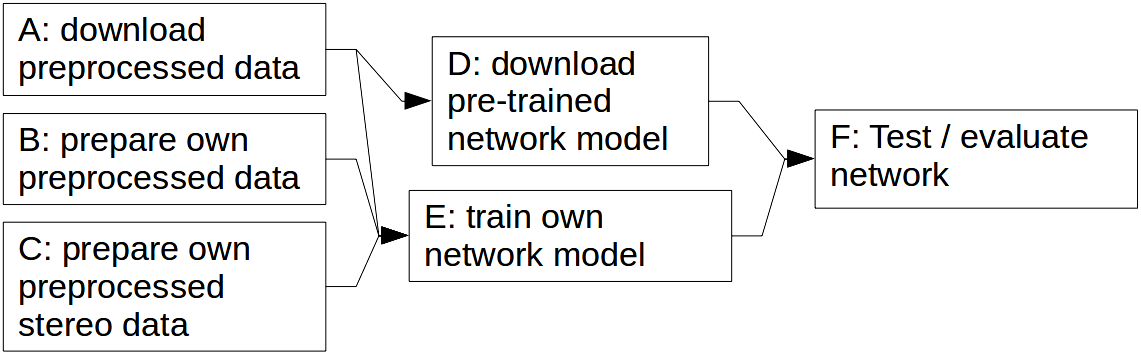
\includegraphics[width=1\textwidth]{../media/fpnet_paths_img.png}
    \caption{Various paths that were planned to simply transition from lidar-based 3D estimation to stereo-based 3D estimation. Generally, paths went chronologically as follow: ADF, AEF, BEF, and finally CEF.}
    \label{fp_paths}
\end{figure}

The most basic path, ADF, is simply using the given model to evaluate and achieve similar results to the official paper. Next, AEF used lidar pointclouds, but the model was trained locally. BEF required locally running the ``preprocessing" step, but was still theoretically identical to the previous two paths. Finally, CEF truly deviates from the other paths by using a stereo-generated pointcloud to preprocess data, then train on that, and finally evaluate the model's detection capability.


% NEWSECTION ===================================================================
\newpage
\section{Procedure / Method}
Now that many of the individual steps of the network have been described above, the complete set of steps taken to produce network estimation will be described. Not every step will be described again, but any deviations from the ``general" usage is clarified. However, this section shall be more detailed in describing how each step was executed.

1. train psmnet on object detection images\\
2. create a preprocessed set of lidar pointclouds generated from PSMnet \\
3. train fpnet on the preprocessed data, according to path CEF as described in Figure \ref{fp_paths} \\
4. test fpnet on the data, specifically focusing on 3D object detection for cars. \\


% NEWSECTION ===================================================================
\newpage
\section{Results}
The raw results of the network training and validation are immediately presented here to quickly provide clarity on the performance of the network, and then these results are to be compared with the performance of other networks and published works.

Firstly, the loss during the Frustum Pointnet training is given in Figure xx. Additionally, the precision-recall curve for the ``Car" class is given as well as the AP score in Figure xx.

Training graph data is in Figure \ref{fpnet_CEFv2_loss_multi}

\begin{figure}[ht]
    \centering
    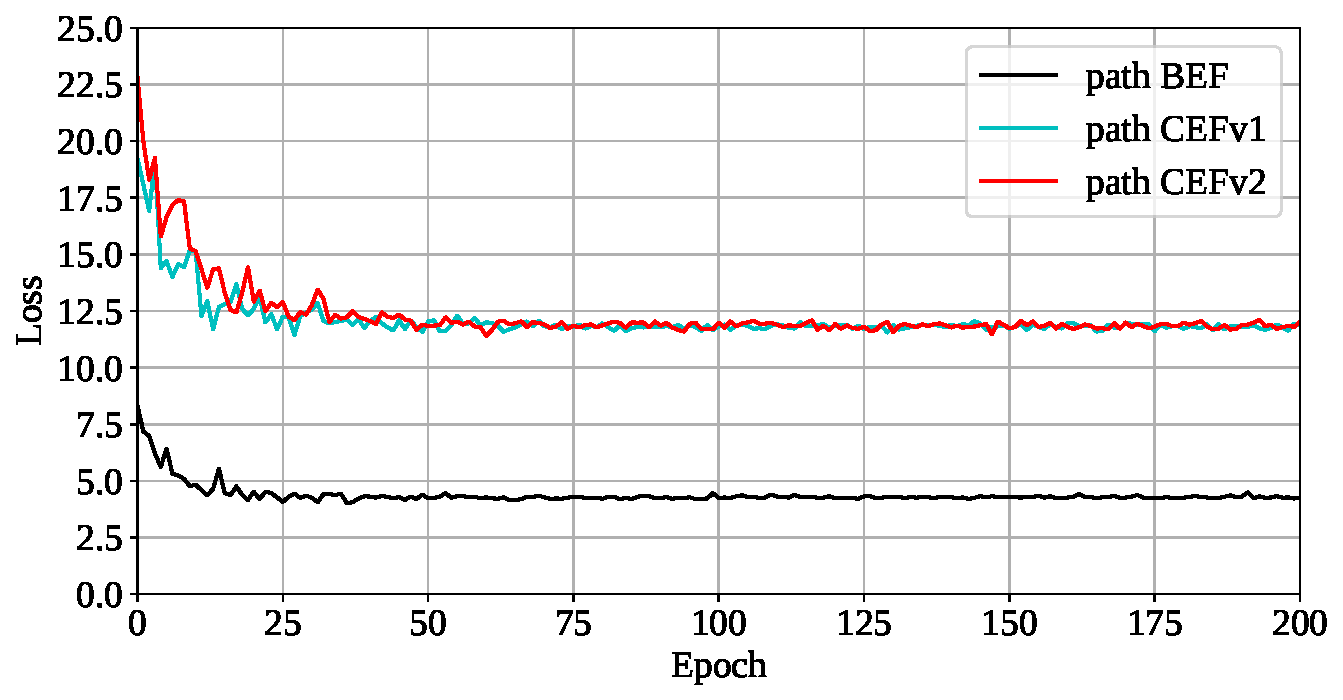
\includegraphics[width=1\textwidth]{../media/fpnet_CEFv2_loss_multi.pdf}
    \caption{texthere xx}
    \label{fpnet_CEFv2_loss_multi}
\end{figure}


% need a precision-recall curve here...
The precision-recall curve for the ``Car" class is below, with AP values included in Figure \ref{fpnet_CEFv2_precrec}.

\begin{figure}[ht]
    \centering
    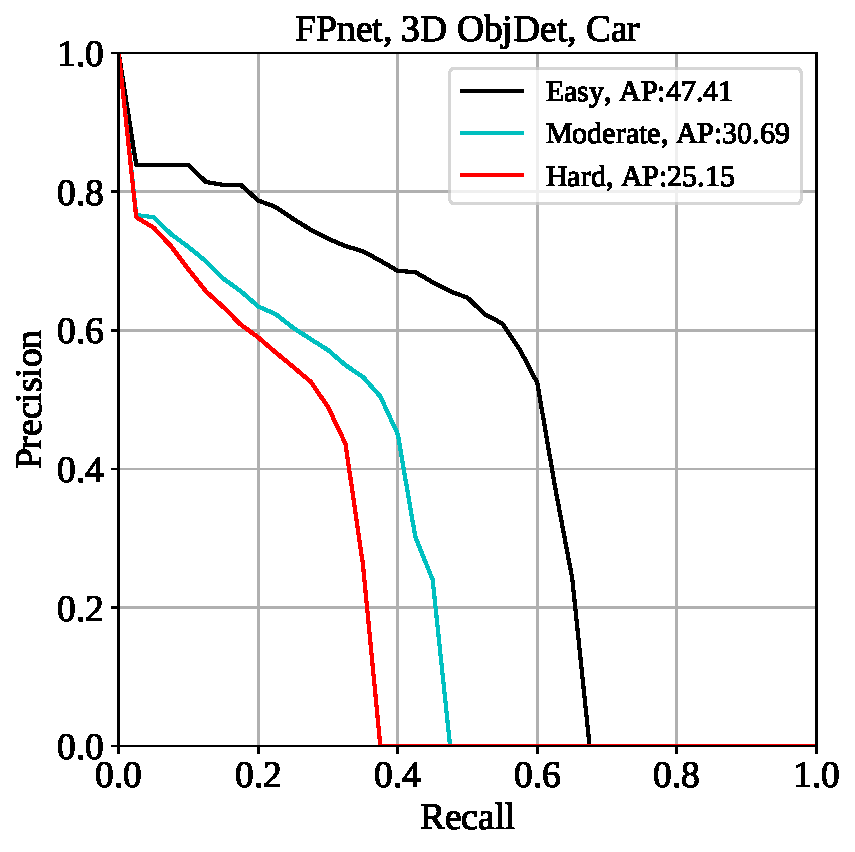
\includegraphics[width=0.6\textwidth]{../media/fpnet_CEFv2_precrec.pdf}
    \caption{texthere xx}
    \label{fpnet_CEFv2_precrec}
\end{figure}

The precision recall results are now plotted against the pseudo lidar paper. They are shown below in Figure \ref{fpnet_CEFv2_precrec_compareWang}.

\begin{figure}[ht]
    \centering
    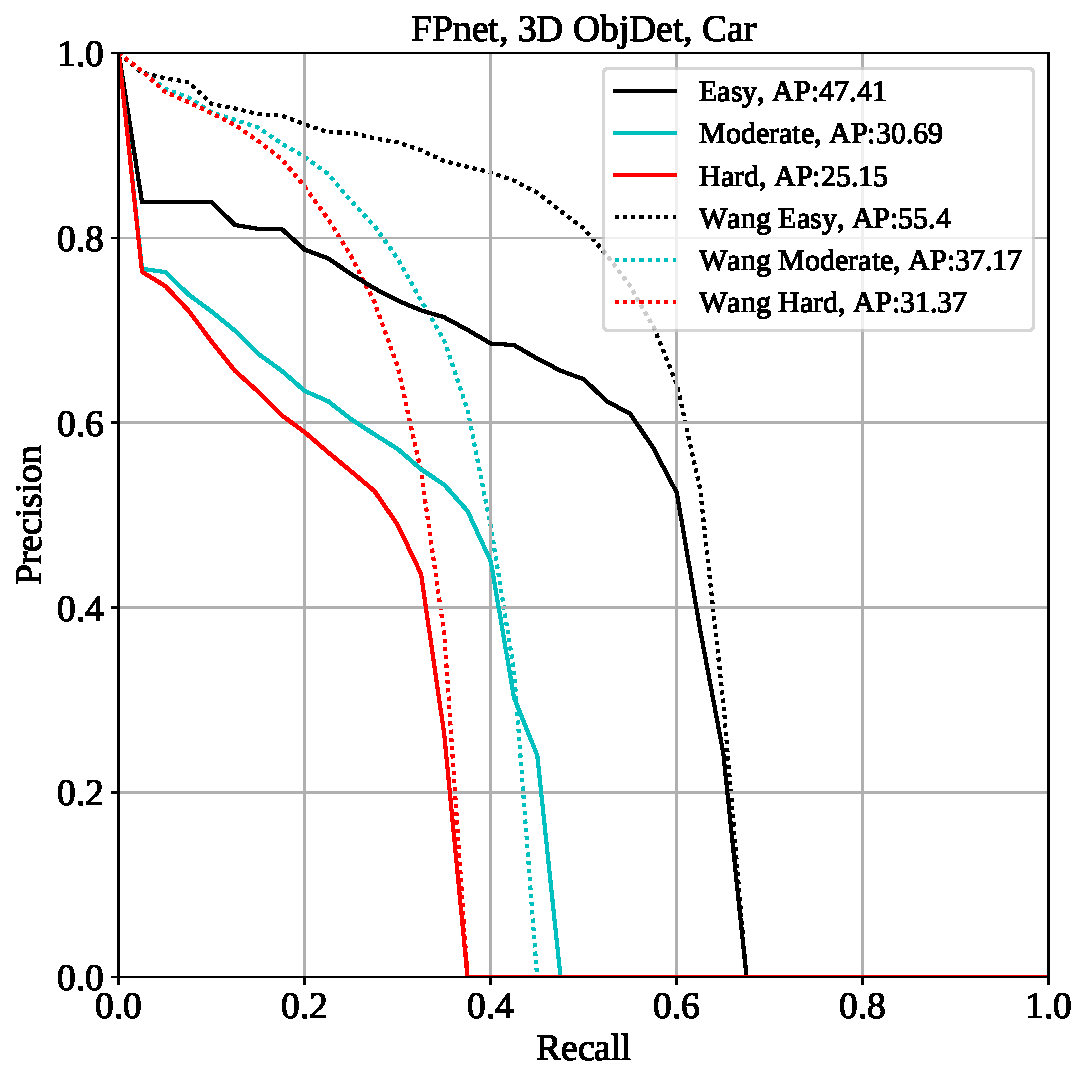
\includegraphics[width=0.6\textwidth]{../media/fpnet_CEFv2_precrec_compareWang.pdf}
    \caption{texthere xx}
    \label{fpnet_CEFv2_precrec_compareWang}
\end{figure}


Comparing our own pr-curve with the results of other papers, namely \cite{wang_pseudo-lidar_2019} and other\_xx, then we find the graph that is seen below in Figure \ref{fpnet_CEFv2_precrec_compareMulti}.



\begin{figure}[ht]
    \centering
    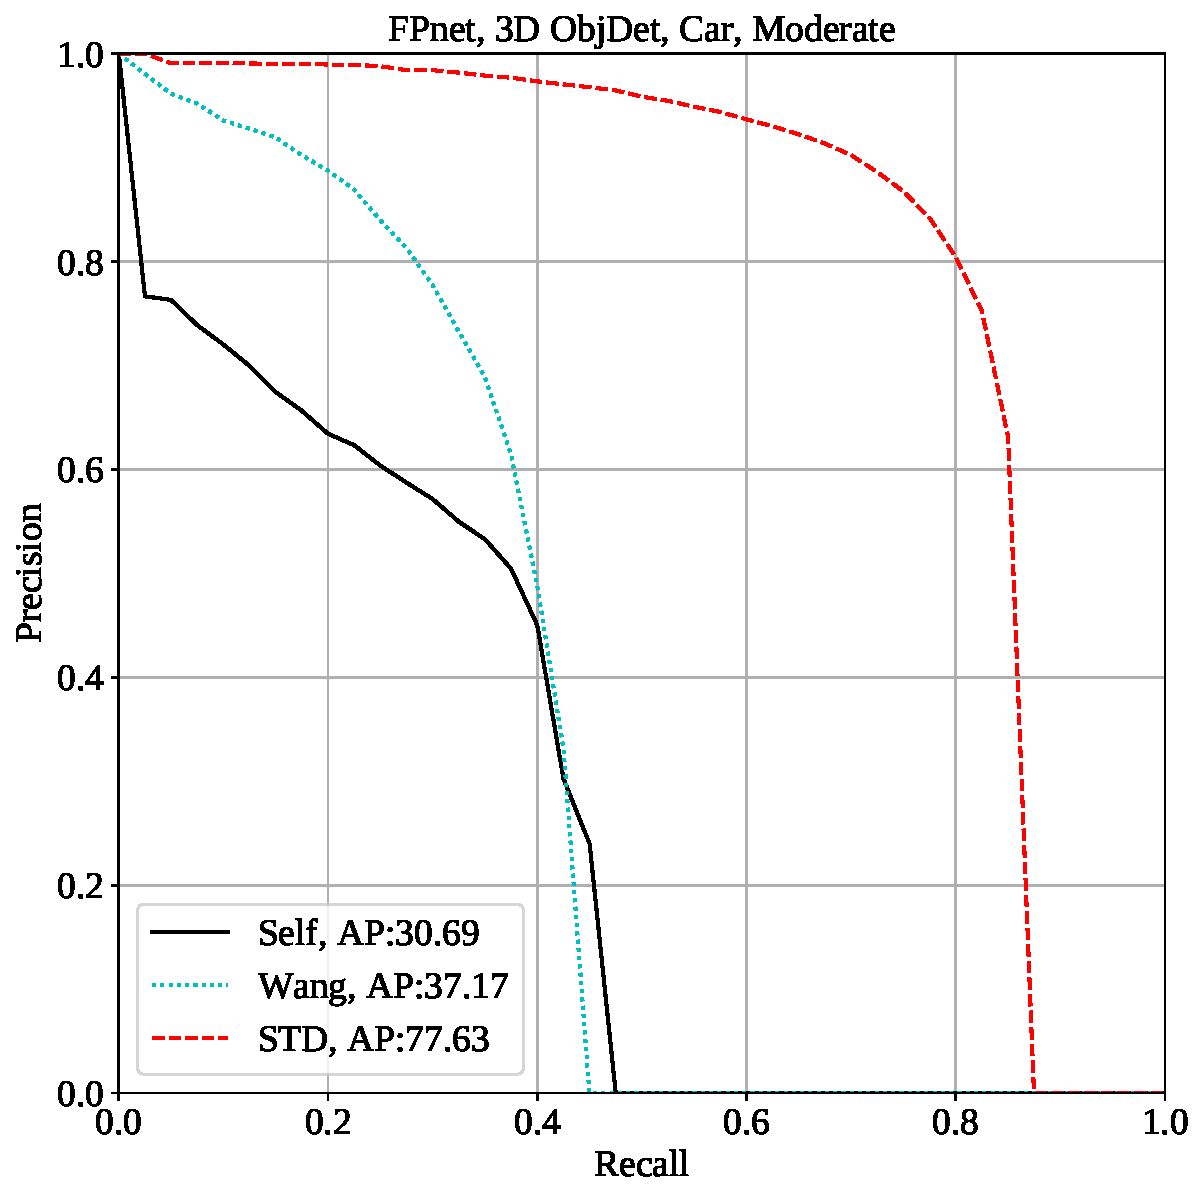
\includegraphics[width=0.6\textwidth]{../media/fpnet_CEFv2_precrec_compareMulti.pdf}
    \caption{texthere xx}
    \label{fpnet_CEFv2_precrec_compareMulti}
\end{figure}

Finally, an examination of the same pr-curves generated on ``easy" criteria yields Figure \ref{fpnet_CEFv2_precrec_compareMulti_easy} below.

\begin{figure}[ht]
    \centering
    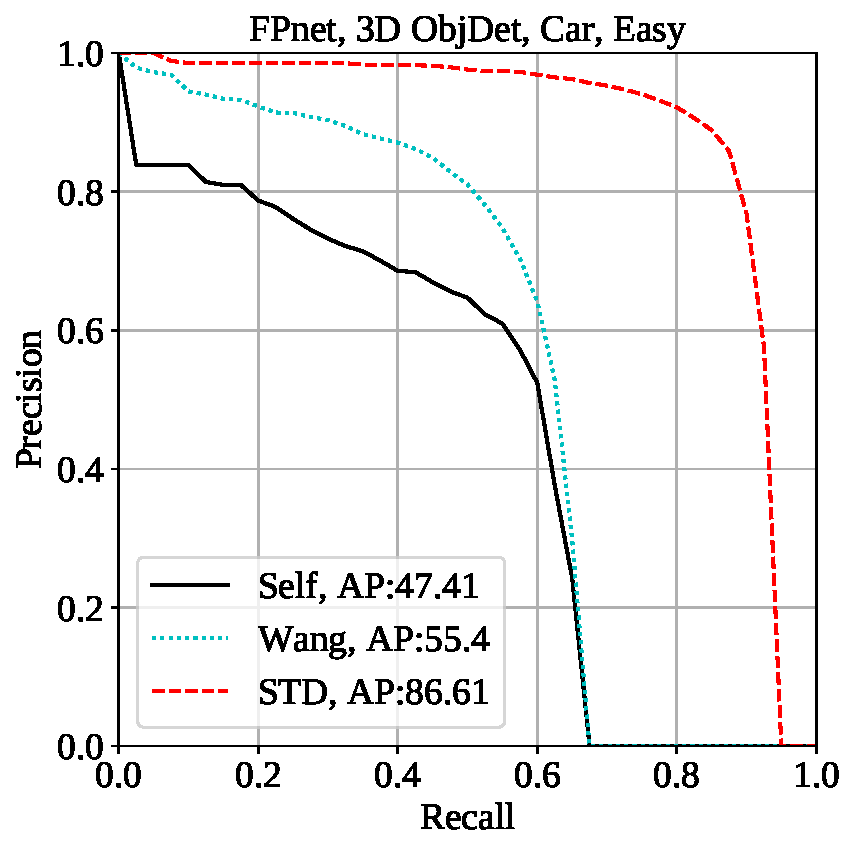
\includegraphics[width=0.6\textwidth]{../media/fpnet_CEFv2_precrec_compareMulti_easy.pdf}
    \caption{texthere xx}
    \label{fpnet_CEFv2_precrec_compareMulti_easy}
\end{figure}


As can be seen from the various graphs, it is clear that although the network does not have the highest performance, it is relatively competitive with other networks of its class.


% NEWSECTION ===================================================================
\newpage
\section{Conclusion}
TextHere xx
